\documentclass[a4paper,12pt]{extarticle}
%\usepackage{fixltx2e}
%\usepackage{newtxtext} % Times New Roman font or alike.
\usepackage[T1]{fontenc}
\usepackage[utf8]{inputenc}

%\usepackage[labelsep=endash]{caption} % Use english in captions instead of Russian
\usepackage{titlesec} % adds dot after section number
\titlelabel{\thetitle.\quad} % adds dot after section number
\usepackage{enumitem} % makes enumerated lists (for indentation adjustment)
\usepackage{indentfirst} % Indent first paragraph
%\usepackage{wrapfig} % Wrapped figures
\usepackage[pdftex]{graphicx} % allows to add figures
\usepackage{subcaption}
\graphicspath{ {figures/} } % figure folder.

\usepackage{amsmath}

\usepackage{amsfonts}
\usepackage{bigints}

\renewcommand{\baselinestretch}{1.0}   % Update line spacing
% Margins of the paper
\usepackage{marginnote} % create notes in the margins with \marginnote{}[3cm]
\usepackage[marginparwidth=20mm, marginparsep=3mm]{geometry}
\geometry{a4paper,
	%total={210mm,297mm}, 
	left=	10mm,
	right=	10mm,
	top=	10mm,
	bottom=	15mm,
}
\usepackage{hyperref}% Adds links to all references.
\newcommand{\bs}{\textbackslash}
\usepackage{color}
\numberwithin{equation}{section}
\usepackage{physics}
\usepackage{nicefrac}
\usepackage{esvect}

% Theorems and Definitions
\usepackage{amsthm}% for Definitions and something else?
\newtheorem{theorem}{Theorem}
\newtheorem{definition}{Definition}[section]
\theoremstyle{remark}
\newtheorem*{remark}{Remark}
\newtheorem*{solution}{Solution}
\newtheorem{exercise}{Exercise}[section]

% Math commands
\newcommand{\vect}[1]{\boldsymbol{#1}}

% Insert a block note
\usepackage{xcolor}
\usepackage[framemethod=default]{mdframed}

\usepackage{CJKutf8}
\usepackage{array}% http://ctan.org/pkg/array
\usepackage{makecell}
\usepackage{longtable}
\begin{document}
\begin{longtable}{|lp{6cm}p{4cm}|}
        \multicolumn{1}{c}{\textbf{Kanji}} & \multicolumn{1}{c}{\textbf{Reading}} & \multicolumn{1}{c}{\textbf{Meaning}} \\ \hline
        \endfirsthead

        \multicolumn{1}{c}{\textbf{Kanji}} & \multicolumn{1}{c}{\textbf{Reading}} & \multicolumn{1}{c}{\textbf{Meaning}} \\ \hline
        \endhead

        \hline
        \endfoot

        \hline \hline
        \endlastfoot

%=============================================
% Row START
%--------------------
% dictionary entry START
\begin{minipage}{0.3\textwidth}
\centerline{
	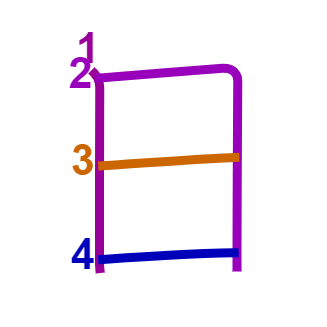
\includegraphics[width=0.4\linewidth,]{nichi}
}
\end{minipage}
&
\begin{CJK}{UTF8}{min}ニチ、ジツ、ひ、-び、-か\end{CJK}
&
day
% dictionary entry END
% Row END
\\ 
%=============================================
% Row START
%--------------------
% dictionary entry START
\begin{minipage}{0.3\textwidth}
\centerline{
	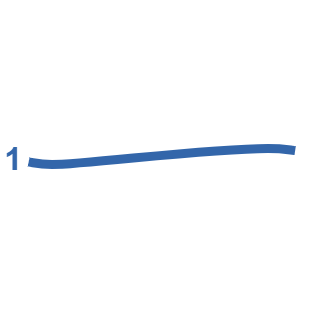
\includegraphics[width=0.4\linewidth,]{ichi}
}
\end{minipage}
&
\begin{CJK}{UTF8}{min}イチ、イツ、ひと-、ひと.つ\end{CJK}
&
one
% dictionary entry END
% Row END
\\ 
%=============================================
% Row START
%--------------------
% dictionary entry START
\begin{minipage}{0.3\textwidth}
\centerline{
	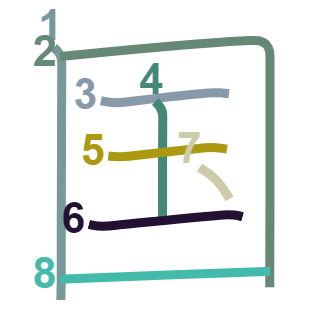
\includegraphics[width=0.4\linewidth,]{kuni}
}
\end{minipage}
&
\begin{CJK}{UTF8}{min}コク、くに\end{CJK}
&
country
% dictionary entry END
% Row END
\\ 
%=============================================
% Row START
%--------------------
% dictionary entry START
\begin{minipage}{0.3\textwidth}
\centerline{
	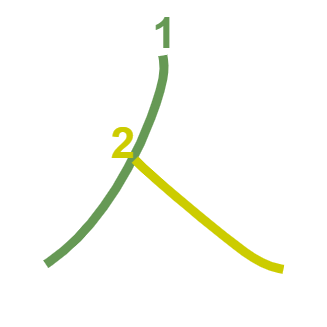
\includegraphics[width=0.4\linewidth,]{hito}
}
\end{minipage}
&
\begin{CJK}{UTF8}{min}ジン、ニン、ひと、-り、-と\end{CJK}
&
person
% dictionary entry END
% Row END
\\ 
%=============================================
% Row START
%--------------------
% dictionary entry START
\begin{minipage}{0.3\textwidth}
\centerline{
	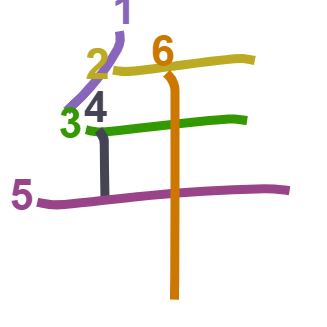
\includegraphics[width=0.4\linewidth,]{nen}
}
\end{minipage}
&
\begin{CJK}{UTF8}{min}ネン、とし\end{CJK}
&
year
% dictionary entry END
% Row END
\\ 
%=============================================
% Row START
%--------------------
% dictionary entry START
\begin{minipage}{0.3\textwidth}
\centerline{
	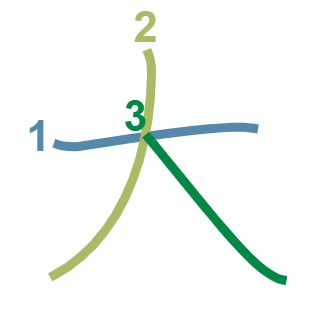
\includegraphics[width=0.4\linewidth,]{dai}
}
\end{minipage}
&
\begin{CJK}{UTF8}{min}ダイ、タイ、おお-、おお.きい、-おお.いに\end{CJK}
&
big
% dictionary entry END
% Row END
\\ 
%=============================================
% Row START
%--------------------
% dictionary entry START
\begin{minipage}{0.3\textwidth}
\centerline{
	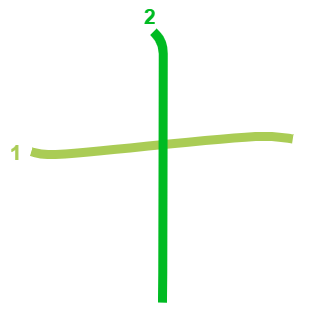
\includegraphics[width=0.4\linewidth,]{jyu}
}
\end{minipage}
&
\begin{CJK}{UTF8}{min}ジュウ、ジッ、ジュッ、とお、と\end{CJK}
&
10
% dictionary entry END
% Row END
\\ 
%=============================================
% Row START
%--------------------
% dictionary entry START
\begin{minipage}{0.3\textwidth}
\centerline{
	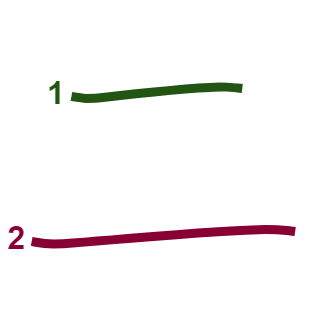
\includegraphics[width=0.4\linewidth,]{ni}
}
\end{minipage}
&
\begin{CJK}{UTF8}{min}ニ、ジ、ふた、ふた.つ、ふたた.び\end{CJK}
&
2
% dictionary entry END
% Row END
\\ 
%=============================================
% Row START
%--------------------
% dictionary entry START
\begin{minipage}{0.3\textwidth}
\centerline{
	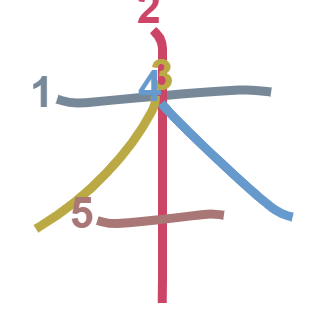
\includegraphics[width=0.4\linewidth,]{hon}
}
\end{minipage}
&
\begin{CJK}{UTF8}{min}ホン、もと\end{CJK}
&
book
% dictionary entry END
% Row END
\\ 
%=============================================
% Row START
%--------------------
% dictionary entry START
\begin{minipage}{0.3\textwidth}
\centerline{
	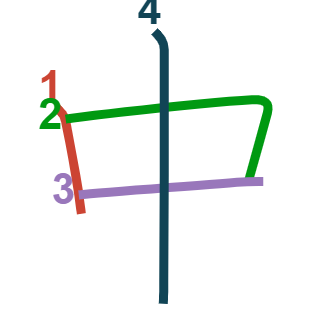
\includegraphics[width=0.4\linewidth,]{naka}
}
\end{minipage}
&
\begin{CJK}{UTF8}{min}チュウ、なか、うち、あた.る\end{CJK}
&
in
% dictionary entry END
% Row END
\\ 
%=============================================
% Row START
%--------------------
% dictionary entry START
\begin{minipage}{0.3\textwidth}
\centerline{
	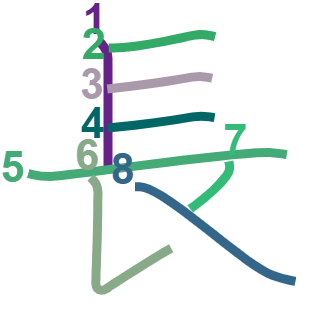
\includegraphics[width=0.4\linewidth,]{nagai}
}
\end{minipage}
&
\begin{CJK}{UTF8}{min}チョウ、なが.い、おさ\end{CJK}
&
long
% dictionary entry END
% Row END
\\ 
%=============================================
% Row START
%--------------------
% dictionary entry START
\begin{minipage}{0.3\textwidth}
\centerline{
	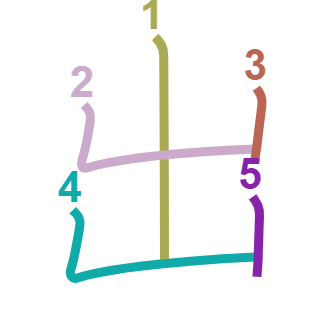
\includegraphics[width=0.4\linewidth,]{deru}
}
\end{minipage}
&
\begin{CJK}{UTF8}{min}シュツ、スイ、で.る、-で、だ.す、-だ.す、い.でる、い.だす\end{CJK}
&
exit
% dictionary entry END
% Row END
\\ 
%=============================================
% Row START
%--------------------
% dictionary entry START
\begin{minipage}{0.3\textwidth}
\centerline{
	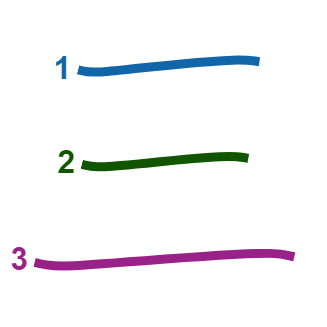
\includegraphics[width=0.4\linewidth,]{san}
}
\end{minipage}
&
\begin{CJK}{UTF8}{min}サン、ゾウ、み、み.つ、みっ.つ\end{CJK}
&
3
% dictionary entry END
% Row END
\\ 
%=============================================
% Row START
%--------------------
% dictionary entry START
\begin{minipage}{0.3\textwidth}
\centerline{
	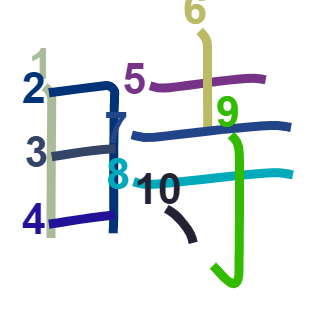
\includegraphics[width=0.4\linewidth,]{toki}
}
\end{minipage}
&
\begin{CJK}{UTF8}{min}ジ、とき、-どき\end{CJK}
&
time
% dictionary entry END
% Row END
\\ 
%=============================================
% Row START
%--------------------
% dictionary entry START
\begin{minipage}{0.3\textwidth}
\centerline{
	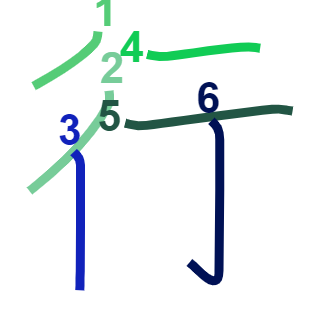
\includegraphics[width=0.4\linewidth,]{iku}
}
\end{minipage}
&
\begin{CJK}{UTF8}{min}コウ、ギョウ、アン、い.く、ゆ.く、-ゆ.き、-ゆき、-い.き、-いき、おこな.う、おこ.なう\end{CJK}
&
to go
% dictionary entry END
% Row END
\\ 
%=============================================
% Row START
%--------------------
% dictionary entry START
\begin{minipage}{0.3\textwidth}
\centerline{
	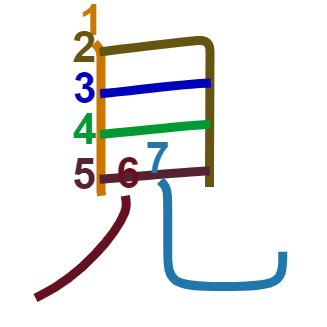
\includegraphics[width=0.4\linewidth,]{miru}
}
\end{minipage}
&
\begin{CJK}{UTF8}{min}ケン、み.る、み.える、み.せる\end{CJK}
&
to see
% dictionary entry END
% Row END
\\ 
%=============================================
% Row START
%--------------------
% dictionary entry START
\begin{minipage}{0.3\textwidth}
\centerline{
	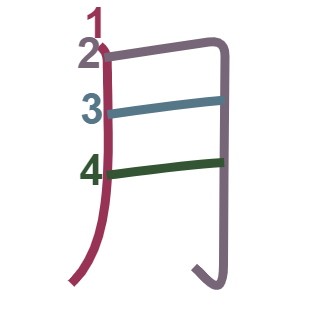
\includegraphics[width=0.4\linewidth,]{tsuki}
}
\end{minipage}
&
\begin{CJK}{UTF8}{min}ゲツ、ガツ、つき\end{CJK}
&
moon
% dictionary entry END
% Row END
\\ 
%=============================================
% Row START
%--------------------
% dictionary entry START
\begin{minipage}{0.3\textwidth}
\centerline{
	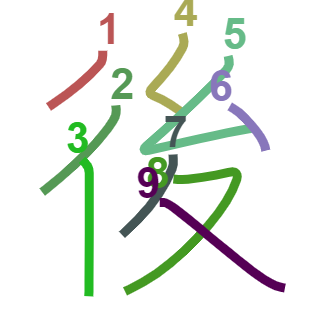
\includegraphics[width=0.4\linewidth,]{ato}
}
\end{minipage}
&
\begin{CJK}{UTF8}{min}ゴ、コウ、のち、うし.ろ、うしろ、あと、おく.れる\end{CJK}
&
behind
% dictionary entry END
% Row END
\\ 
%=============================================
% Row START
%--------------------
% dictionary entry START
\begin{minipage}{0.3\textwidth}
\centerline{
	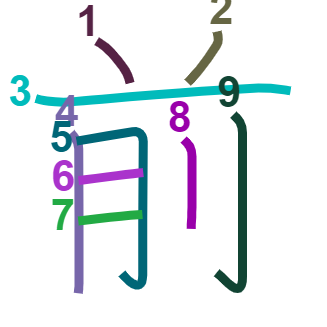
\includegraphics[width=0.4\linewidth,]{mae}
}
\end{minipage}
&
\begin{CJK}{UTF8}{min}ゼン、まえ、-まえ\end{CJK}
&
infront
% dictionary entry END
% Row END
\\ 
%=============================================
% Row START
%--------------------
% dictionary entry START
\begin{minipage}{0.3\textwidth}
\centerline{
	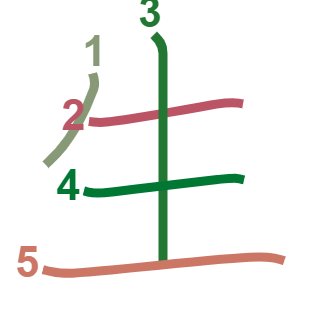
\includegraphics[width=0.4\linewidth,]{ikiru}
}
\end{minipage}
&
\begin{CJK}{UTF8}{min} セイ、 ショウ、 い.きる、 い.かす、 い.ける、 う.まれる、 うま.れる、 う.まれ、 うまれ、 う.む、 お.う、 は.える、 は.やす、 き 、 なま、 なま-、 な.る、 な.す、 む.す\end{CJK}
&
 to live
% dictionary entry END
% Row END
\\ 
%=============================================
% Row START
%--------------------
% dictionary entry START
\begin{minipage}{0.3\textwidth}
\centerline{
	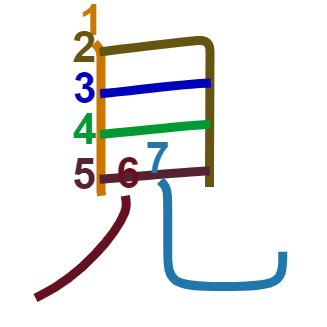
\includegraphics[width=0.4\linewidth,]{go}
}
\end{minipage}
&
\begin{CJK}{UTF8}{min} ゴ 、いつ 、いつ.つ\end{CJK}
&
 5
% dictionary entry END
% Row END
\\ 
%=============================================
% Row START
%--------------------
% dictionary entry START
\begin{minipage}{0.3\textwidth}
\centerline{
	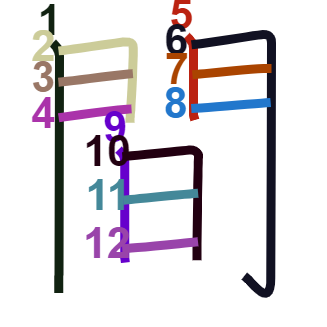
\includegraphics[width=0.4\linewidth,]{aida}
}
\end{minipage}
&
\begin{CJK}{UTF8}{min} カン 、ケン 、あいだ 、 ま 、あい\end{CJK}
&
 between
% dictionary entry END
% Row END
\\ 
%=============================================
% Row START
%--------------------
% dictionary entry START
\begin{minipage}{0.3\textwidth}
\centerline{
	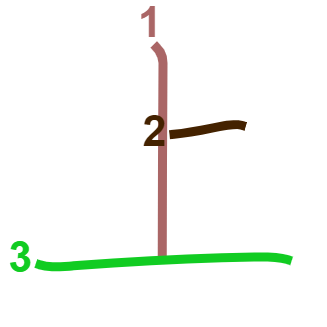
\includegraphics[width=0.4\linewidth,]{ue}
}
\end{minipage}
&
\begin{CJK}{UTF8}{min} ジョウ 、ショウ 、シャン 、うえ 、-うえ  、うわ- 、かみ 、あ.げる 、 -あ.げる 、あ.がる 、 -あ.がる 、あ.がり 、 -あ.がり 、のぼ.る 、 のぼ.り 、のぼ.せる 、 のぼ.す 、よ.す\end{CJK}
&
 up
% dictionary entry END
% Row END
\\ 
%=============================================
% Row START
%--------------------
% dictionary entry START
\begin{minipage}{0.3\textwidth}
\centerline{
	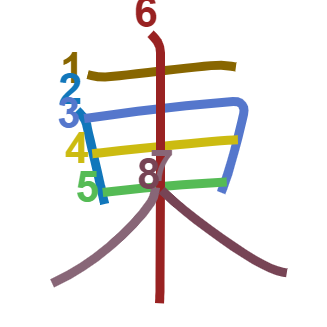
\includegraphics[width=0.4\linewidth,]{higashi}
}
\end{minipage}
&
\begin{CJK}{UTF8}{min} トウ 、ひがし\end{CJK}
&
 east
% dictionary entry END
% Row END
\\ 
%=============================================
% Row START
%--------------------
% dictionary entry START
\begin{minipage}{0.3\textwidth}
\centerline{
	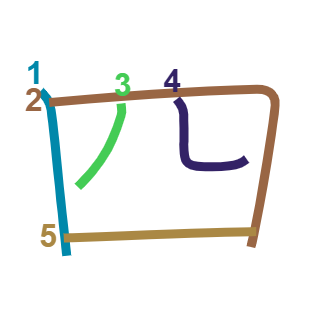
\includegraphics[width=0.4\linewidth,]{yon}
}
\end{minipage}
&
\begin{CJK}{UTF8}{min} シ 、よ 、よ.つ 、よっ.つ 、よん\end{CJK}
&
 4
% dictionary entry END
% Row END
\\ 
%=============================================
% Row START
%--------------------
% dictionary entry START
\begin{minipage}{0.3\textwidth}
\centerline{
	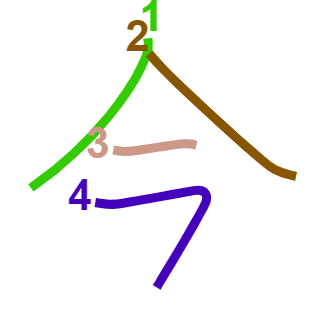
\includegraphics[width=0.4\linewidth,]{ima}
}
\end{minipage}
&
\begin{CJK}{UTF8}{min} コン 、キン 、いま\end{CJK}
&
 now
% dictionary entry END
% Row END
\\ 
%=============================================
% Row START
%--------------------
% dictionary entry START
\begin{minipage}{0.3\textwidth}
\centerline{
	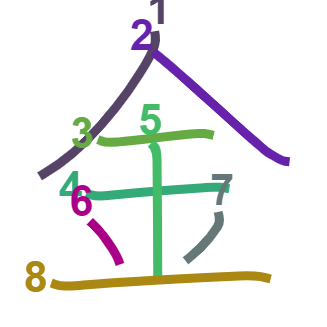
\includegraphics[width=0.4\linewidth,]{kane}
}
\end{minipage}
&
\begin{CJK}{UTF8}{min} キン 、コン 、ゴン  、かね 、かな- 、-がね\end{CJK}
&
 gold
% dictionary entry END
% Row END
\\ 
%=============================================
% Row START
%--------------------
% dictionary entry START
\begin{minipage}{0.3\textwidth}
\centerline{
	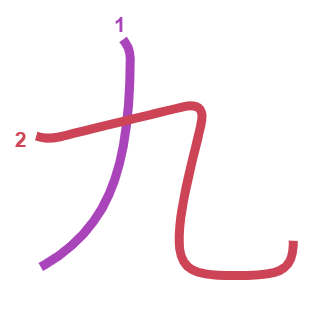
\includegraphics[width=0.4\linewidth,]{kyu}
}
\end{minipage}
&
\begin{CJK}{UTF8}{min} キュウ 、ク 、ここの 、 ここの.つ\end{CJK}
&
 9
% dictionary entry END
% Row END
\\ 
%=============================================
% Row START
%--------------------
% dictionary entry START
\begin{minipage}{0.3\textwidth}
\centerline{
	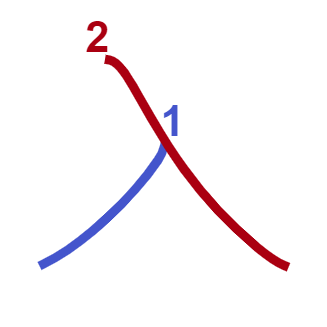
\includegraphics[width=0.4\linewidth,]{iru}
}
\end{minipage}
&
\begin{CJK}{UTF8}{min} ニュウ 、ジュ 、い.る 、 -い.る 、-い.り 、い.れる 、-い.れ 、はい.る\end{CJK}
&
 insert
% dictionary entry END
% Row END
\\ 
%=============================================
% Row START
%--------------------
% dictionary entry START
\begin{minipage}{0.3\textwidth}
\centerline{
	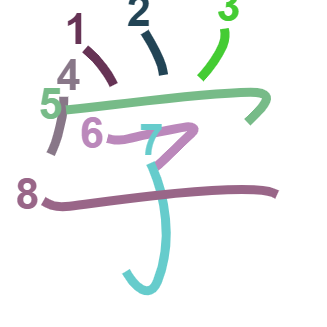
\includegraphics[width=0.4\linewidth,]{manabu}
}
\end{minipage}
&
\begin{CJK}{UTF8}{min}ガク 、まな.ぶ\end{CJK}
&
 to study
% dictionary entry END
% Row END
\\ 
%=============================================
% Row START
%--------------------
% dictionary entry START
\begin{minipage}{0.3\textwidth}
\centerline{
	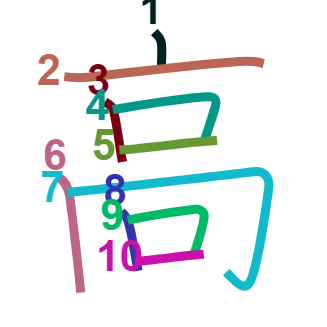
\includegraphics[width=0.4\linewidth,]{takai}
}
\end{minipage}
&
\begin{CJK}{UTF8}{min} コウ 、たか.い 、たか 、 -だか 、たか.まる  、たか.める\end{CJK}
&
 high
% dictionary entry END
% Row END
\\ 
%=============================================
% Row START
%--------------------
% dictionary entry START
\begin{minipage}{0.3\textwidth}
\centerline{
	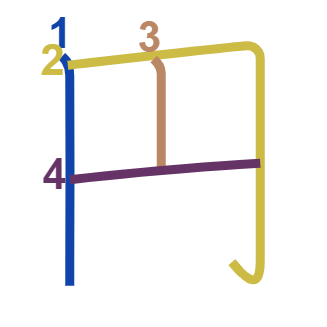
\includegraphics[width=0.4\linewidth,]{en}
}
\end{minipage}
&
\begin{CJK}{UTF8}{min} エン 、まる.い 、まる 、 まど 、まど.か 、まろ.やか\end{CJK}
&
 round
% dictionary entry END
% Row END
\\ 
%=============================================
% Row START
%--------------------
% dictionary entry START
\begin{minipage}{0.3\textwidth}
\centerline{
	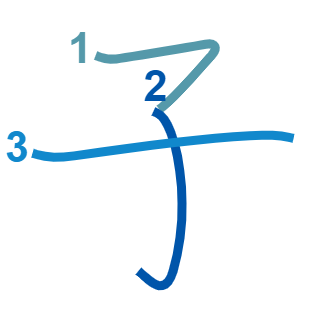
\includegraphics[width=0.4\linewidth,]{ko}
}
\end{minipage}
&
\begin{CJK}{UTF8}{min} シ 、ス 、ツ 、こ 、-こ 、ね\end{CJK}
&
 child; 11PM-1AM
% dictionary entry END
% Row END
\\ 
%=============================================
% Row START
%--------------------
% dictionary entry START
\begin{minipage}{0.3\textwidth}
\centerline{
	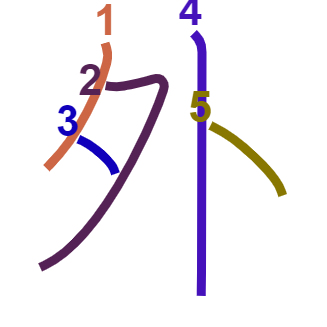
\includegraphics[width=0.4\linewidth,]{soto}
}
\end{minipage}
&
\begin{CJK}{UTF8}{min} ガイ 、ゲ 、そと 、ほか 、はず.す 、はず.れる 、と-\end{CJK}
&
 outside
% dictionary entry END
% Row END
\\ 
%=============================================
% Row START
%--------------------
% dictionary entry START
\begin{minipage}{0.3\textwidth}
\centerline{
	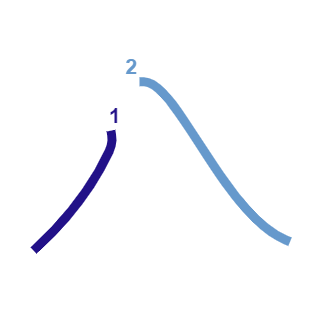
\includegraphics[width=0.4\linewidth,]{hachi}
}
\end{minipage}
&
\begin{CJK}{UTF8}{min} ハチ 、や 、や.つ 、やっ.つ 、よう\end{CJK}
&
 8
% dictionary entry END
% Row END
\\ 
%=============================================
% Row START
%--------------------
% dictionary entry START
\begin{minipage}{0.3\textwidth}
\centerline{
	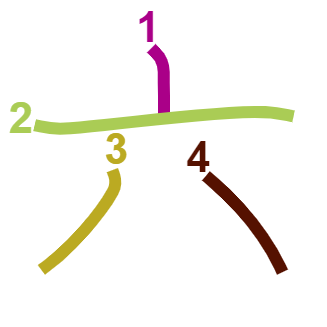
\includegraphics[width=0.4\linewidth,]{roku}
}
\end{minipage}
&
\begin{CJK}{UTF8}{min} ロク 、リク 、む 、む.つ 、むっ.つ 、むい\end{CJK}
&
 6
% dictionary entry END
% Row END
\\ 
%=============================================
% Row START
%--------------------
% dictionary entry START
\begin{minipage}{0.3\textwidth}
\centerline{
	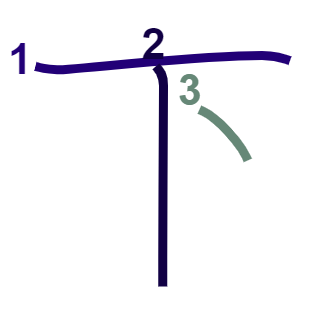
\includegraphics[width=0.4\linewidth,]{shita}
}
\end{minipage}
&
\begin{CJK}{UTF8}{min} カ 、ゲ 、した 、しも 、 もと 、さ.げる 、さ.がる 、くだ.る 、くだ.り 、くだ.す 、-くだ.す 、くだ.さる 、お.ろす 、お.りる\end{CJK}
&
 down
% dictionary entry END
% Row END
\\ 
%=============================================
% Row START
%--------------------
% dictionary entry START
\begin{minipage}{0.3\textwidth}
\centerline{
	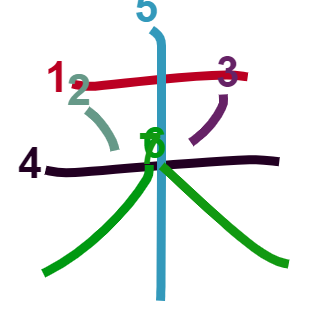
\includegraphics[width=0.4\linewidth,]{kome}
}
\end{minipage}
&
\begin{CJK}{UTF8}{min} ライ 、タイ 、く.る 、きた.る 、きた.す 、き.たす 、き.たる 、き 、こ\end{CJK}
&
 rice
% dictionary entry END
% Row END
\\ 
%=============================================
% Row START
%--------------------
% dictionary entry START
\begin{minipage}{0.3\textwidth}
\centerline{
	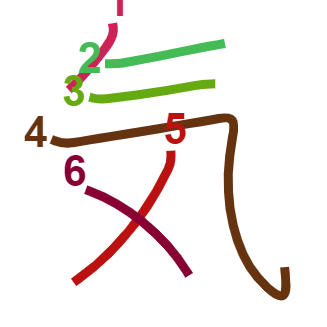
\includegraphics[width=0.4\linewidth,]{ki}
}
\end{minipage}
&
\begin{CJK}{UTF8}{min} キ 、ケ 、いき\end{CJK}
&
 spirit
% dictionary entry END
% Row END
\\ 
%=============================================
% Row START
%--------------------
% dictionary entry START
\begin{minipage}{0.3\textwidth}
\centerline{
	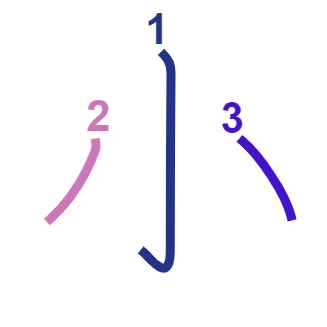
\includegraphics[width=0.4\linewidth,]{chisai}
}
\end{minipage}
&
\begin{CJK}{UTF8}{min} ショウ 、ちい.さい 、こ- 、お- 、さ-\end{CJK}
&
 small
% dictionary entry END
% Row END
\\ 
%=============================================
% Row START
%--------------------
% dictionary entry START
\begin{minipage}{0.3\textwidth}
\centerline{
	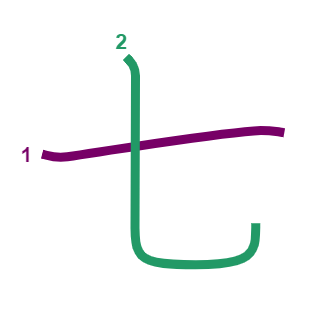
\includegraphics[width=0.4\linewidth,]{nana}
}
\end{minipage}
&
\begin{CJK}{UTF8}{min} シチ 、なな 、なな.つ 、 なの\end{CJK}
&
 7
% dictionary entry END
% Row END
\\ 
%=============================================
% Row START
%--------------------
% dictionary entry START
\begin{minipage}{0.3\textwidth}
\centerline{
	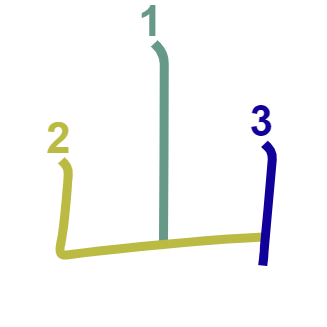
\includegraphics[width=0.4\linewidth,]{yama}
}
\end{minipage}
&
\begin{CJK}{UTF8}{min} サン 、セン 、やま\end{CJK}
&
 mountain
% dictionary entry END
% Row END
\\ 
%=============================================
% Row START
%--------------------
% dictionary entry START
\begin{minipage}{0.3\textwidth}
\centerline{
	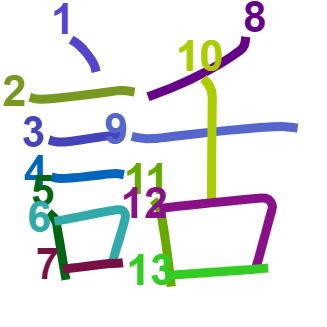
\includegraphics[width=0.4\linewidth,]{hanashi}
}
\end{minipage}
&
\begin{CJK}{UTF8}{min} ワ 、はな.す 、はなし\end{CJK}
&
 tale
% dictionary entry END
% Row END
\\ 
%=============================================
% Row START
%--------------------
% dictionary entry START
\begin{minipage}{0.3\textwidth}
\centerline{
	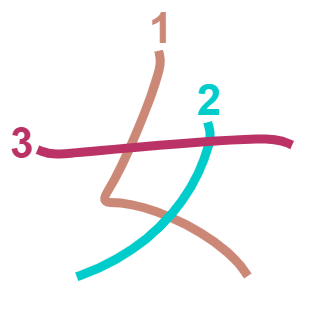
\includegraphics[width=0.4\linewidth,]{onna}
}
\end{minipage}
&
\begin{CJK}{UTF8}{min} ジョ 、ニョ 、ニョウ 、 おんな 、め\end{CJK}
&
 woman
% dictionary entry END
% Row END
\\ 
%=============================================
% Row START
%--------------------
% dictionary entry START
\begin{minipage}{0.3\textwidth}
\centerline{
	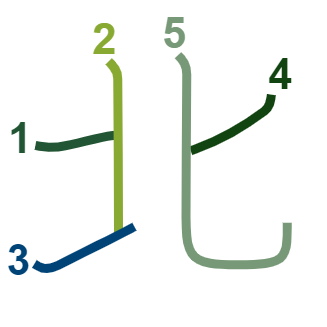
\includegraphics[width=0.4\linewidth,]{kita}
}
\end{minipage}
&
\begin{CJK}{UTF8}{min} ホク 、きた\end{CJK}
&
 north
% dictionary entry END
% Row END
\\ 
%=============================================
% Row START
%--------------------
% dictionary entry START
\begin{minipage}{0.3\textwidth}
\centerline{
	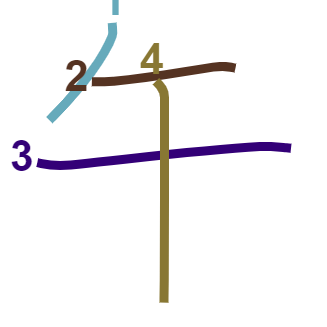
\includegraphics[width=0.4\linewidth,]{uma}
}
\end{minipage}
&
\begin{CJK}{UTF8}{min} ゴ 、うま\end{CJK}
&
 noon
% dictionary entry END
% Row END
\\ 
%=============================================
% Row START
%--------------------
% dictionary entry START
\begin{minipage}{0.3\textwidth}
\centerline{
	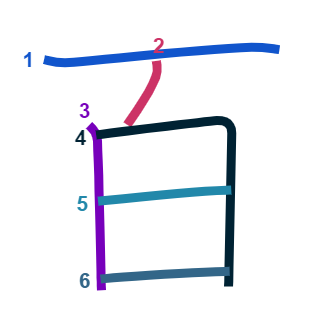
\includegraphics[width=0.4\linewidth,]{hyaku}
}
\end{minipage}
&
\begin{CJK}{UTF8}{min} ヒャク 、ビャク 、もも\end{CJK}
&
 100
% dictionary entry END
% Row END
\\ 
%=============================================
% Row START
%--------------------
% dictionary entry START
\begin{minipage}{0.3\textwidth}
\centerline{
	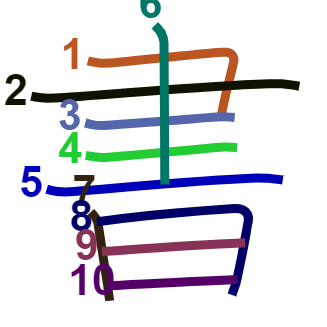
\includegraphics[width=0.4\linewidth,]{kaku}
}
\end{minipage}
&
\begin{CJK}{UTF8}{min} ショ 、か.く 、-が.き 、 -がき\end{CJK}
&
 to write
% dictionary entry END
% Row END
\\ 
%=============================================
% Row START
%--------------------
% dictionary entry START
\begin{minipage}{0.3\textwidth}
\centerline{
	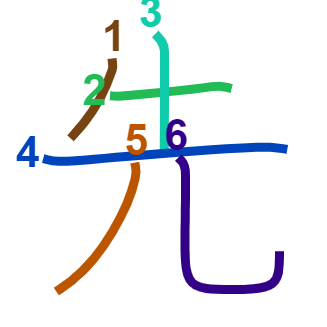
\includegraphics[width=0.4\linewidth,]{sama}
}
\end{minipage}
&
\begin{CJK}{UTF8}{min} セン 、さき 、ま.ず\end{CJK}
&
 before; ahead
% dictionary entry END
% Row END
\\ 
%=============================================
% Row START
%--------------------
% dictionary entry START
\begin{minipage}{0.3\textwidth}
\centerline{
	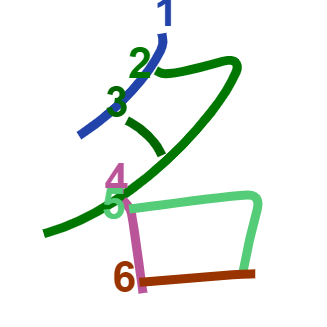
\includegraphics[width=0.4\linewidth,]{na}
}
\end{minipage}
&
\begin{CJK}{UTF8}{min}メイ 、ミョウ 、な 、-な\end{CJK}
&
 name
% dictionary entry END
% Row END
\\ 
%=============================================
% Row START
%--------------------
% dictionary entry START
\begin{minipage}{0.3\textwidth}
\centerline{
	\includegraphics[width=0.4\linewidth,]{kawa}
}
\end{minipage}
&
\begin{CJK}{UTF8}{min} セン 、かわ\end{CJK}
&
 stream; river
% dictionary entry END
% Row END
\\ 
%=============================================
% Row START
%--------------------
% dictionary entry START
\begin{minipage}{0.3\textwidth}
\centerline{
	\includegraphics[width=0.4\linewidth,]{sen}
}
\end{minipage}
&
\begin{CJK}{UTF8}{min} セン 、ち\end{CJK}
&
 1000
% dictionary entry END
% Row END
\\ 
%=============================================
% Row START
%--------------------
% dictionary entry START
\begin{minipage}{0.3\textwidth}
\centerline{
	\includegraphics[width=0.4\linewidth,]{mizu}
}
\end{minipage}
&
\begin{CJK}{UTF8}{min} スイ 、みず 、みず-\end{CJK}
&
 water
% dictionary entry END
% Row END
\\ 
%=============================================
% Row START
%--------------------
% dictionary entry START
\begin{minipage}{0.3\textwidth}
\centerline{
	\includegraphics[width=0.4\linewidth,]{han}
}
\end{minipage}
&
\begin{CJK}{UTF8}{min}ハン 、なか.ば\end{CJK}
&
 half
% dictionary entry END
% Row END
\\ 
%=============================================
% Row START
%--------------------
% dictionary entry START
\begin{minipage}{0.3\textwidth}
\centerline{
	\includegraphics[width=0.4\linewidth,]{otoko}
}
\end{minipage}
&
\begin{CJK}{UTF8}{min}ダン 、ナン 、おとこ 、 お\end{CJK}
&
 man
% dictionary entry END
% Row END
\\ 
%=============================================
% Row START
%--------------------
% dictionary entry START
\begin{minipage}{0.3\textwidth}
\centerline{
	\includegraphics[width=0.4\linewidth,]{nishi}
}
\end{minipage}
&
\begin{CJK}{UTF8}{min} セイ 、サイ 、ス 、にし\end{CJK}
&
 west
% dictionary entry END
% Row END
\\ 
%=============================================
% Row START
%--------------------
% dictionary entry START
\begin{minipage}{0.3\textwidth}
\centerline{
	\includegraphics[width=0.4\linewidth,]{den}
}
\end{minipage}
&
\begin{CJK}{UTF8}{min}デン\end{CJK}
&
 electricity
% dictionary entry END
% Row END
\\ 
%=============================================
% Row START
%--------------------
% dictionary entry START
\begin{minipage}{0.3\textwidth}
\centerline{
	\includegraphics[width=0.4\linewidth,]{koutest}
}
\end{minipage}
&
\begin{CJK}{UTF8}{min} コウ 、キョウ\end{CJK}
&
exam; school; printing; proof; correction
% dictionary entry END
% Row END
\\ 
%=============================================
% Row START
%--------------------
% dictionary entry START
\begin{minipage}{0.3\textwidth}
\centerline{
	\includegraphics[width=0.4\linewidth,]{kataru}
}
\end{minipage}
&
\begin{CJK}{UTF8}{min} ゴ 、かた.る 、かた.らう\end{CJK}
&
 word
% dictionary entry END
% Row END
\\ 
%=============================================
% Row START
%--------------------
% dictionary entry START
\begin{minipage}{0.3\textwidth}
\centerline{
	\includegraphics[width=0.4\linewidth,]{tsuchi}
}
\end{minipage}
&
\begin{CJK}{UTF8}{min} ド 、ト 、つち\end{CJK}
&
 soil; earth
% dictionary entry END
% Row END
\\ 
%=============================================
% Row START
%--------------------
% dictionary entry START
\begin{minipage}{0.3\textwidth}
\centerline{
	\includegraphics[width=0.4\linewidth,]{kitree}
}
\end{minipage}
&
\begin{CJK}{UTF8}{min} ボク 、モク 、き 、こ-\end{CJK}
&
 tree
% dictionary entry END
% Row END
\\ 
%=============================================
% Row START
%--------------------
% dictionary entry START
\begin{minipage}{0.3\textwidth}
\centerline{
	\includegraphics[width=0.4\linewidth,]{kiku}
}
\end{minipage}
&
\begin{CJK}{UTF8}{min} ブン 、モン 、き.く 、き.こえる\end{CJK}
&
 to hear
% dictionary entry END
% Row END
\\ 
%=============================================
% Row START
%--------------------
% dictionary entry START
\begin{minipage}{0.3\textwidth}
\centerline{
	\includegraphics[width=0.4\linewidth,]{taberu}
}
\end{minipage}
&
\begin{CJK}{UTF8}{min} ショク 、ジキ 、く.う 、 く.らう 、た.べる 、は.む\end{CJK}
&
 to eat
% dictionary entry END
% Row END
\\ 
%=============================================
% Row START
%--------------------
% dictionary entry START
\begin{minipage}{0.3\textwidth}
\centerline{
	\includegraphics[width=0.4\linewidth,]{kuruma}
}
\end{minipage}
&
\begin{CJK}{UTF8}{min} シャ 、くるま\end{CJK}
&
 car
% dictionary entry END
% Row END
\\ 
%=============================================
% Row START
%--------------------
% dictionary entry START
\begin{minipage}{0.3\textwidth}
\centerline{
	\includegraphics[width=0.4\linewidth,]{nani}
}
\end{minipage}
&
\begin{CJK}{UTF8}{min} カ 、なに 、なん 、なに- 、なん-\end{CJK}
&
 what
% dictionary entry END
% Row END
\\ 
%=============================================
% Row START
%--------------------
% dictionary entry START
\begin{minipage}{0.3\textwidth}
\centerline{
	\includegraphics[width=0.4\linewidth,]{minami}
}
\end{minipage}
&
\begin{CJK}{UTF8}{min} ナン 、ナ 、みなみ\end{CJK}
&
 south
% dictionary entry END
% Row END
\\ 
%=============================================
% Row START
%--------------------
% dictionary entry START
\begin{minipage}{0.3\textwidth}
\centerline{
	\includegraphics[width=0.4\linewidth,]{man}
}
\end{minipage}
&
\begin{CJK}{UTF8}{min} マン 、バン 、よろず\end{CJK}
&
 $10^{4}$
% dictionary entry END
% Row END
\\ 
%=============================================
% Row START
%--------------------
% dictionary entry START
\begin{minipage}{0.3\textwidth}
\centerline{
	\includegraphics[width=0.4\linewidth,]{goto}
}
\end{minipage}
&
\begin{CJK}{UTF8}{min} マイ 、ごと 、-ごと.に\end{CJK}
&
 every
% dictionary entry END
% Row END
\\ 
%=============================================
% Row START
%--------------------
% dictionary entry START
\begin{minipage}{0.3\textwidth}
\centerline{
	\includegraphics[width=0.4\linewidth,]{shiro}
}
\end{minipage}
&
\begin{CJK}{UTF8}{min} ハク 、ビャク 、しろ 、 しら- 、しろ.い\end{CJK}
&
 white
% dictionary entry END
% Row END
\\ 
%=============================================
% Row START
%--------------------
% dictionary entry START
\begin{minipage}{0.3\textwidth}
\centerline{
	\includegraphics[width=0.4\linewidth,]{ten}
}
\end{minipage}
&
\begin{CJK}{UTF8}{min} テン 、あまつ 、あめ 、 あま-\end{CJK}
&
 sky
% dictionary entry END
% Row END
\\ 
%=============================================
% Row START
%--------------------
% dictionary entry START
\begin{minipage}{0.3\textwidth}
\centerline{
	\includegraphics[width=0.4\linewidth,]{haha}
}
\end{minipage}
&
\begin{CJK}{UTF8}{min} ボ 、はは 、も\end{CJK}
&
 mother
% dictionary entry END
% Row END
\\ 
%=============================================
% Row START
%--------------------
% dictionary entry START
\begin{minipage}{0.3\textwidth}
\centerline{
	\includegraphics[width=0.4\linewidth,]{hi}
}
\end{minipage}
&
\begin{CJK}{UTF8}{min} カ 、ひ 、-び 、ほ-\end{CJK}
&
 fire
% dictionary entry END
% Row END
\\ 
%=============================================
% Row START
%--------------------
% dictionary entry START
\begin{minipage}{0.3\textwidth}
\centerline{
	\includegraphics[width=0.4\linewidth,]{migi}
}
\end{minipage}
&
\begin{CJK}{UTF8}{min} ウ 、ユウ 、みぎ\end{CJK}
&
 right
% dictionary entry END
% Row END
\\ 
%=============================================
% Row START
%--------------------
% dictionary entry START
\begin{minipage}{0.3\textwidth}
\centerline{
	\includegraphics[width=0.4\linewidth,]{yomu}
}
\end{minipage}
&
\begin{CJK}{UTF8}{min} ドク 、トク 、トウ 、よ.む 、-よ.み\end{CJK}
&
 to read
% dictionary entry END
% Row END
\\ 
%=============================================
% Row START
%--------------------
% dictionary entry START
\begin{minipage}{0.3\textwidth}
\centerline{
	\includegraphics[width=0.4\linewidth,]{tomo}
}
\end{minipage}
&
\begin{CJK}{UTF8}{min} ユウ 、とも\end{CJK}
&
friend
% dictionary entry END
% Row END
\\ 
%=============================================
% Row START
%--------------------
% dictionary entry START
\begin{minipage}{0.3\textwidth}
\centerline{
	\includegraphics[width=0.4\linewidth,]{hidari}
}
\end{minipage}
&
\begin{CJK}{UTF8}{min} サ 、シャ 、ひだり\end{CJK}
&
 left
% dictionary entry END
% Row END
\\ 
%=============================================
% Row START
%--------------------
% dictionary entry START
\begin{minipage}{0.3\textwidth}
\centerline{
	\includegraphics[width=0.4\linewidth,]{yasumu}
}
\end{minipage}
&
\begin{CJK}{UTF8}{min} キュウ 、やす.む 、やす.まる 、やす.める\end{CJK}
&
 to rest
% dictionary entry END
% Row END
\\ 
%=============================================
% Row START
%--------------------
% dictionary entry START
\begin{minipage}{0.3\textwidth}
\centerline{
	\includegraphics[width=0.4\linewidth,]{chichi}
}
\end{minipage}
&
\begin{CJK}{UTF8}{min}フ 、ちち\end{CJK}
&
 father
% dictionary entry END
% Row END
\\ 
%=============================================
% Row START
%--------------------
% dictionary entry START
\begin{minipage}{0.3\textwidth}
\centerline{
	\includegraphics[width=0.4\linewidth,]{ame}
}
\end{minipage}
&
\begin{CJK}{UTF8}{min} ウ 、あめ 、あま- 、-さめ\end{CJK}
&
 rain
% dictionary entry END
% Row END
\\ 
%=============================================
\end{longtable}\end{document}\n